% ------------------------------------------------------------------------------
% TYPO3 CMS 7.4 - What's New (English Version)
%
% @author	Michael Schams <schams.net>
% @license	Creative Commons BY-NC-SA 3.0
% @link		http://typo3.org/download/release-notes/whats-new/
% @language	English
% ------------------------------------------------------------------------------
% LTXE-CHAPTER-UID:		0dbe76ce-5948c314-454b95fd-543cb62c
% LTXE-CHAPTER-NAME:	Backend User Interface
% ------------------------------------------------------------------------------

\section{Interfaccia utente Backend}
\begin{frame}[fragile]
	\frametitle{Interfaccia utente Backend}

	\begin{center}\huge{Capitolo 1:}\end{center}
	\begin{center}\huge{\color{typo3darkgrey}\textbf{Interfaccia utente Backend}}\end{center}

\end{frame}

% ------------------------------------------------------------------------------
% LTXE-SLIDE-START
% LTXE-SLIDE-UID:		1d13abab-2905e884-08c4fe07-8e6c5067
% LTXE-SLIDE-ORIGIN:	464d4ba6-dab07499-0cd5f168-552e9729 English
% LTXE-SLIDE-ORIGIN:	8080f469-3c5592f0-dc25ad87-894c2648 German
% LTXE-SLIDE-TITLE:		Feature: #48947 - Avatars for backend users
% LTXE-SLIDE-REFERENCE:	Feature-48947-AvatarsForBackendUsers.rst
% ------------------------------------------------------------------------------
\begin{frame}[fragile]
	\frametitle{Interfaccia utente Backend}
	\framesubtitle{Avatars per gli utenti di backend}

	Per migliorare i riscontri dell'utente nelle modifiche condivise dei contenuti, gli utenti di backend possono utilizzare un avatar.
	Le piccole immagini degli utenti sono visualizzate nella topbar, nella lista utenti e in altri posti.

	\begin{figure}
		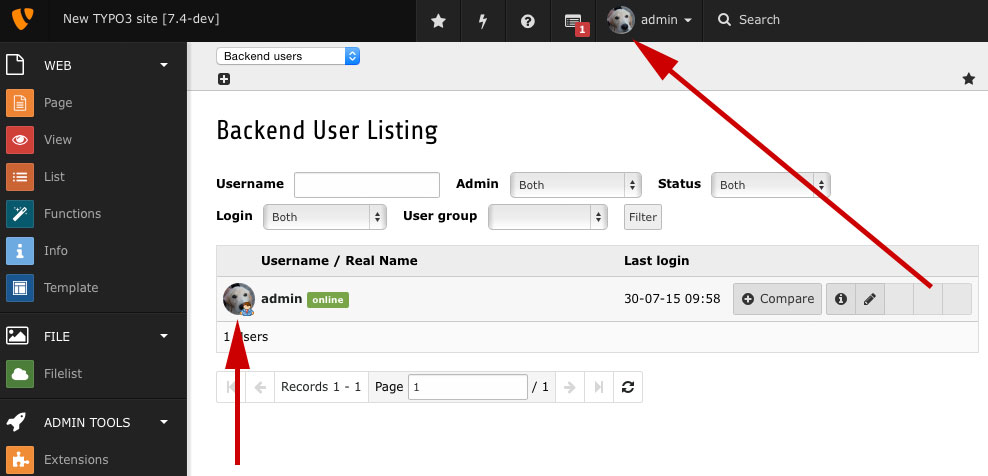
\includegraphics[width=0.9\linewidth]{BackendUserInterface/48947.jpg}
	\end{figure}

\end{frame}

% ------------------------------------------------------------------------------
% LTXE-SLIDE-START
% LTXE-SLIDE-UID:		eca240fb-a619b87b-b26758b7-cd1cb581
% LTXE-SLIDE-ORIGIN:	89f348c8-db045eff-5dfc4f42-da1a2cfa English
% LTXE-SLIDE-ORIGIN:	b0f7e15a-7cc72aaa-79738ec7-643c5cec German
% LTXE-SLIDE-TITLE:		Feature: #56133 - Replace file feature for fal file list
% LTXE-SLIDE-REFERENCE:	Feature-56133-ReplaceFileFeatureForFalFileList.rst
% ------------------------------------------------------------------------------
\begin{frame}[fragile]
	\frametitle{Interfaccia utente Backend}
	\framesubtitle{Sostituzione file}

	I file nella lista dei record FAL possono essere \textbf{sostituiti} (necessaria l'attivazione della "vista estesa").
	Il nome di un file esistente può essere mantenuto o aggiornato.

	\begin{figure}
		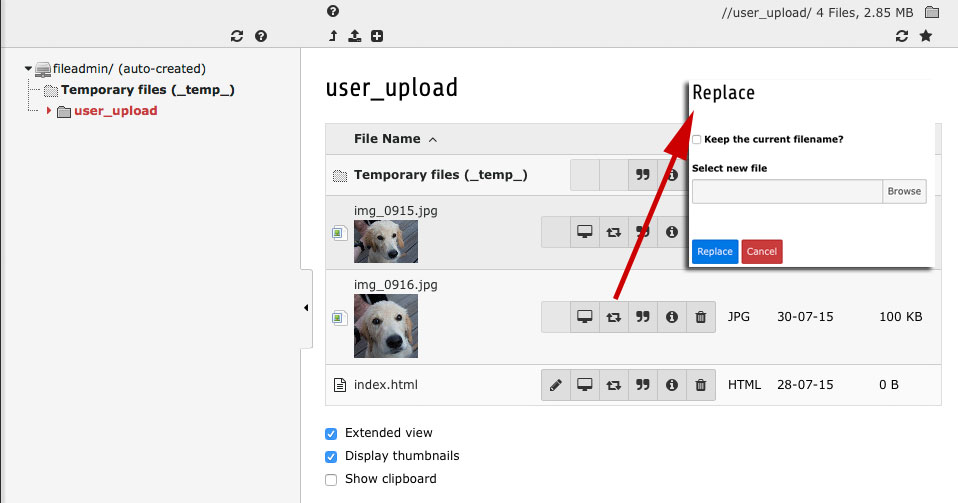
\includegraphics[width=0.75\linewidth]{BackendUserInterface/56133.jpg}
	\end{figure}

\end{frame}

% ------------------------------------------------------------------------------
% LTXE-SLIDE-START
% LTXE-SLIDE-UID:		256ee39e-2b681f96-7e3c2107-eeb82353
% LTXE-SLIDE-ORIGIN:	7e5987f7-9a91ea61-8564c721-0f8d5e4a English
% LTXE-SLIDE-ORIGIN:	613354cc-9475feef-bec620c5-31170549 German
% LTXE-SLIDE-TITLE:		Feature: #67574 - Display online status in backend user list
% LTXE-SLIDE-REFERENCE:	Feature-67574-DisplayOnlineStatusInBackendUserList.rst
% ------------------------------------------------------------------------------
\begin{frame}[fragile]
	\frametitle{Interfaccia utente Backend}
	\framesubtitle{Stato online degli utenti di backend}

	Lo stato online degli utenti di backend è visibile nel modulo "Utenti di backend".

	\begin{figure}
		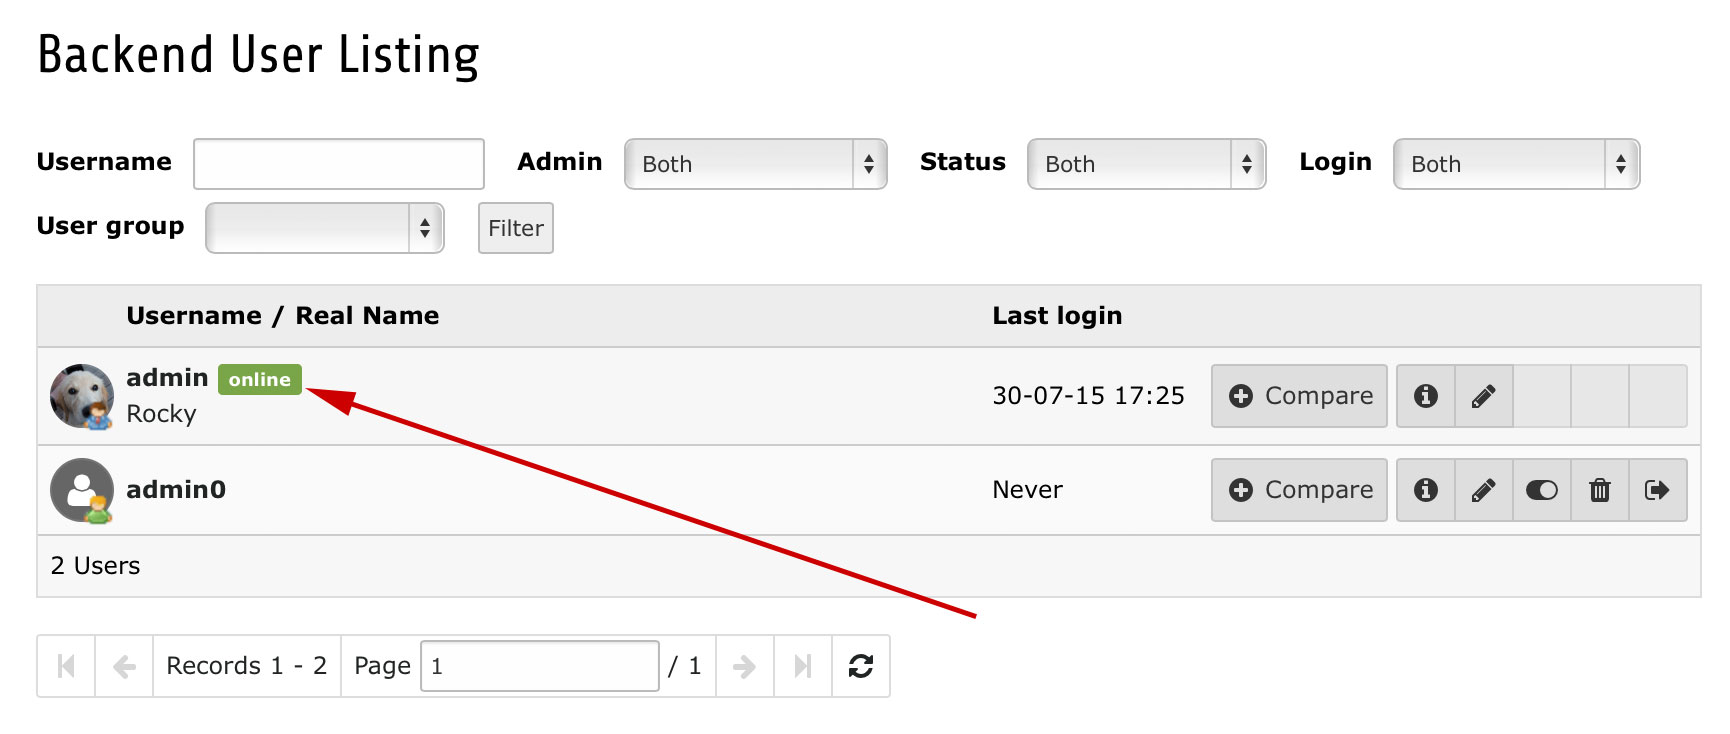
\includegraphics[width=0.9\linewidth]{BackendUserInterface/67574.jpg}
	\end{figure}

\end{frame}

% ------------------------------------------------------------------------------
% LTXE-SLIDE-START
% LTXE-SLIDE-UID:		302a1cd8-3049ec75-cf657272-bc9839b0
% LTXE-SLIDE-ORIGIN:	0154fc51-74683590-ebbe8559-ce6a0d57 English
% LTXE-SLIDE-ORIGIN:	00c93fe2-9d128591-20b71814-13556f43 German
% LTXE-SLIDE-TITLE:		FormEngine: Drop "Show secondary options"
% LTXE-SLIDE-REFERENCE:	https://forge.typo3.org/issues/67753
% ------------------------------------------------------------------------------
\begin{frame}[fragile]
	\frametitle{Interfaccia utente Backend}
	\framesubtitle{Rimosso "Opzioni secondarie"}

	Il checkbox "Opzioni secondarie (palette)", l'opzione di pagina TSconfig \texttt{options.enableShowPalettes}
	e l'impostazione TCA sono stati rimossi. Le impostazioni sono sempre visibili e non possono più essere nascoste.

	\begin{figure}
		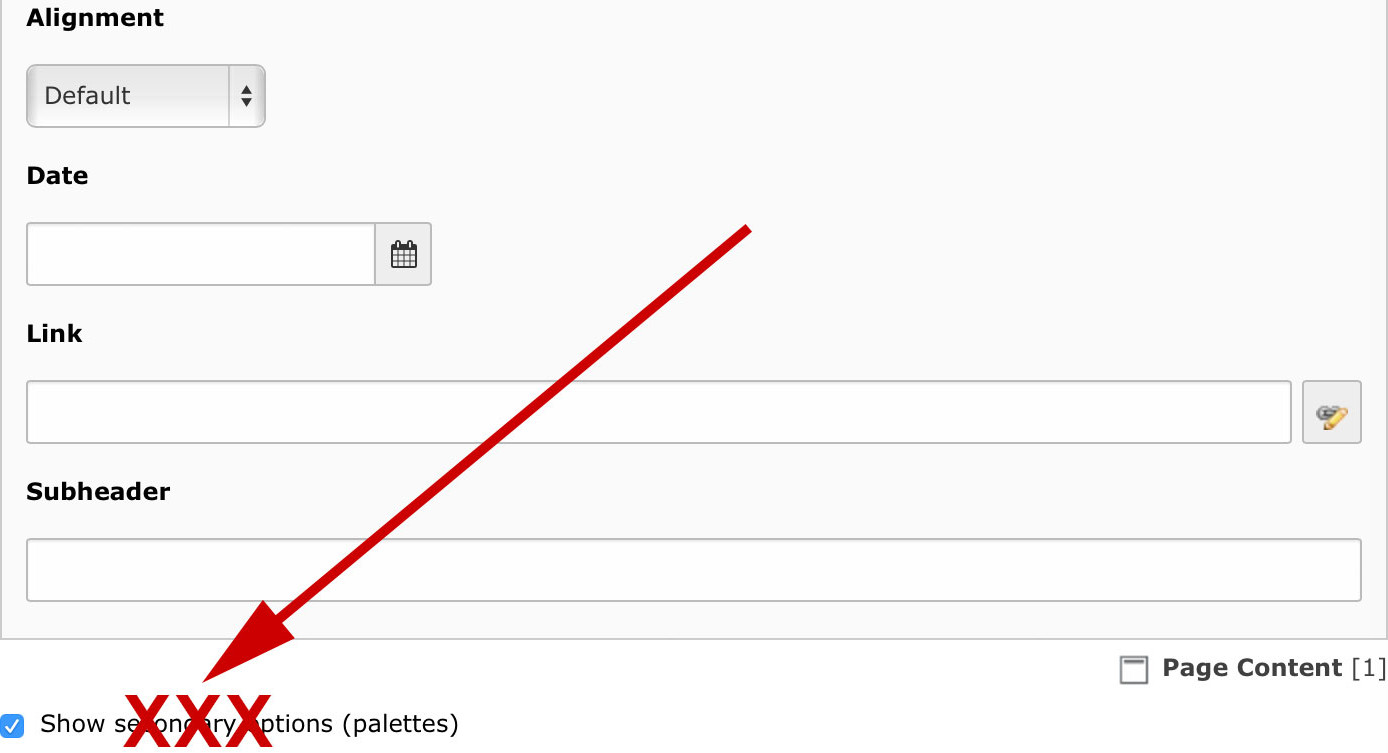
\includegraphics[width=0.7\linewidth]{BackendUserInterface/67753.jpg}
	\end{figure}

\end{frame}

% ------------------------------------------------------------------------------
% LTXE-SLIDE-START
% LTXE-SLIDE-UID:		92d6e47b-92d97c82-6b19ac0c-c91341ee
% LTXE-SLIDE-ORIGIN:	f9b24e36-28e8872c-41297de9-52467554 English
% LTXE-SLIDE-ORIGIN:	bab4e93d-0a6d4612-41b2f67e-47c37ff7 German
% LTXE-SLIDE-TITLE:		Feature: #67578 - Add description-field for backend-users
% LTXE-SLIDE-REFERENCE:	Feature-67578-AddDescriptionFieldForBeUsers.rst
% ------------------------------------------------------------------------------
\begin{frame}[fragile]
	\frametitle{Interfaccia utente Backend}
	\framesubtitle{Descrizione per gli utenti di backend}

	Un nuovo campo "Descrizione" è stato aggiunto ai record degli utenti di backend.

	\begin{figure}
		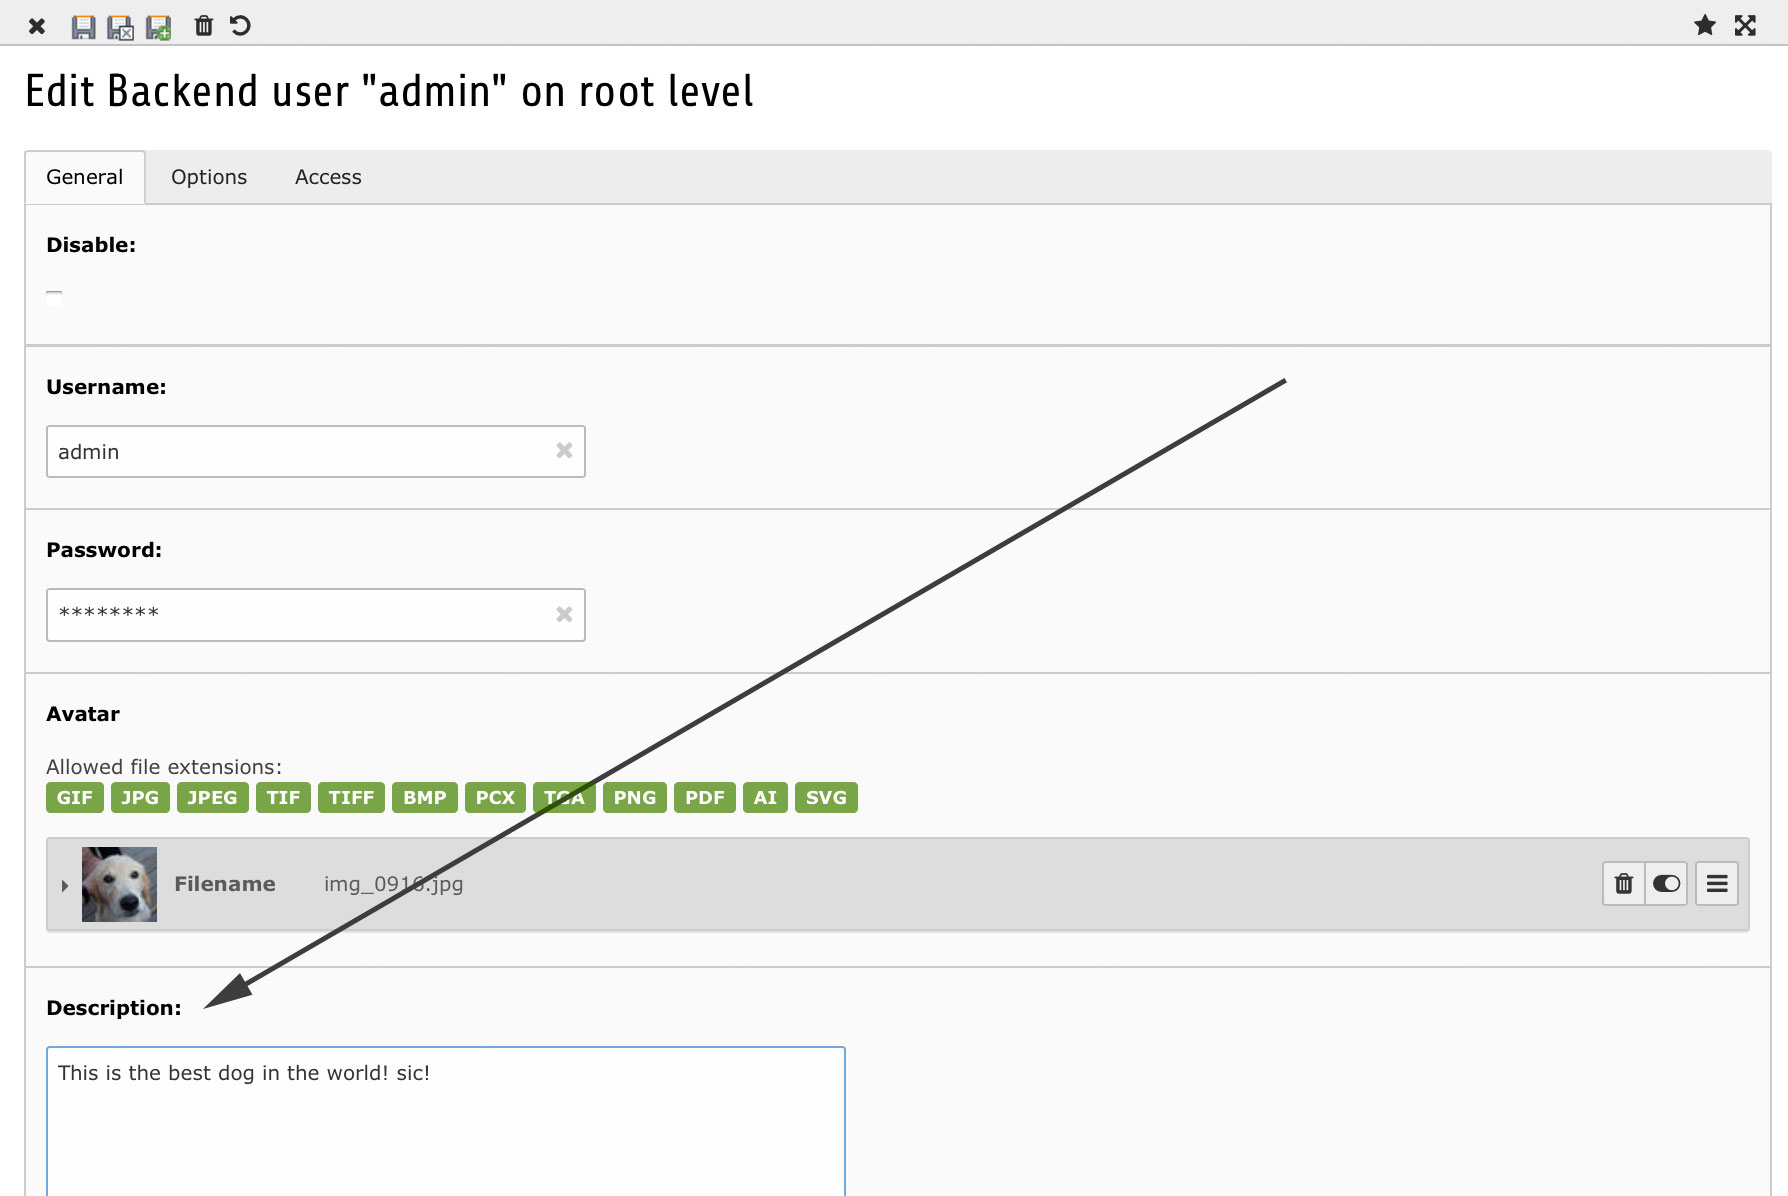
\includegraphics[width=0.7\linewidth]{BackendUserInterface/67578.jpg}
	\end{figure}

\end{frame}

% ------------------------------------------------------------------------------
% LTXE-SLIDE-START
% LTXE-SLIDE-UID:		07fd1aa4-f07f5199-034f6f39-03c759cc
% LTXE-SLIDE-ORIGIN:	83db5442-fa2edfcc-925dd5b6-4afe26f5 English
% LTXE-SLIDE-ORIGIN:	649bd9ee-240381c8-950424ea-f032775b German
% LTXE-SLIDE-TITLE:		Feature: #67603 - Introduce TCA > ctrl > descriptionColumn
% LTXE-SLIDE-REFERENCE:	Feature-67603-IntroduceTcaDescriptionColumn.rst
% ------------------------------------------------------------------------------
\begin{frame}[fragile]
	\frametitle{Interfaccia utente Backend}
	\framesubtitle{Colonna descrizione per le tabelle}

	Configurando una colonna (solitamente \texttt{description}) nelle impostazioni TCA \texttt{['TCA']['ctrl']['descriptionColumn']},
	è mostrata una descrizione (può migliorare l'usabilità per gli editori e gli amministratori).

	\begin{figure}
		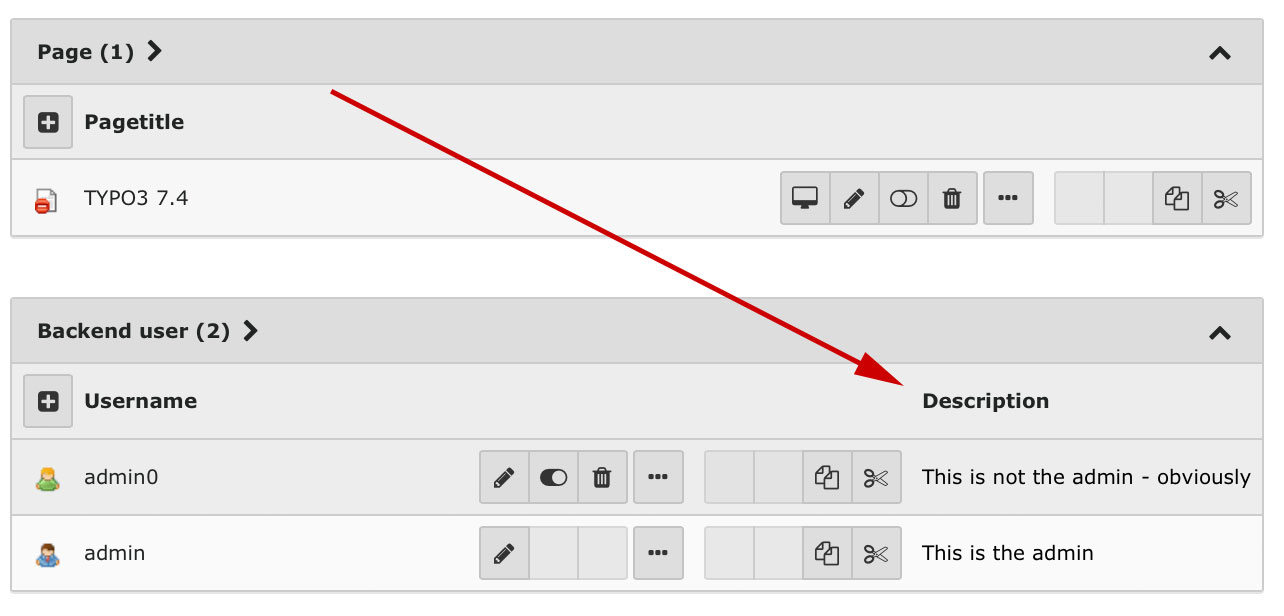
\includegraphics[width=0.7\linewidth]{BackendUserInterface/67603.jpg}
	\end{figure}

\end{frame}

% ------------------------------------------------------------------------------
% LTXE-SLIDE-START
% LTXE-SLIDE-UID:		48db6f57-612eb6ef-a436cc52-9534cdd1
% LTXE-SLIDE-ORIGIN:	7c5400a9-c4b667f3-1a0c046a-9dd3b6a9 English
% LTXE-SLIDE-ORIGIN:	2eeaec46-1929743b-8e6f9285-13d20d3c German
% LTXE-SLIDE-TITLE:		Feature: #59570 - Add description-field for filemounts
% LTXE-SLIDE-REFERENCE:	Feature-59570-AddDescriptionFieldForFilemounts.rst
% ------------------------------------------------------------------------------
\begin{frame}[fragile]
	\frametitle{Interfaccia utente Backend}
	\framesubtitle{Descrizione per Filemounts}

	Un nuovo campo "Descrizione" è stato aggiunto ai record filemount.
	Il campo permette agli amministratori di aggiungere una breve descrizione sull'utilizzo del filemount,
	quali documenti dovrebbe contenere, ecc.

	\begin{figure}
		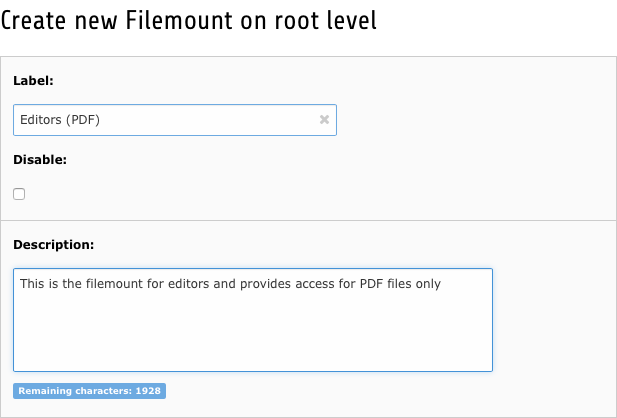
\includegraphics[width=0.55\linewidth]{BackendUserInterface/59570.png}
	\end{figure}

\end{frame}

% ------------------------------------------------------------------------------
% LTXE-SLIDE-START
% LTXE-SLIDE-UID:		1dd60758-e41128a5-f9050320-1c7c1c72
% LTXE-SLIDE-ORIGIN:	d00f63c4-05272792-21a0a301-4d6a726c English
% LTXE-SLIDE-ORIGIN:	879b1dda-9167d830-373f7457-0391ebee German
% LTXE-SLIDE-TITLE:		Feature: #68197 - Show a dialog for existing files on upload
% LTXE-SLIDE-REFERENCE:	Feature-68197-ShowADialogForExistingFilesOnUpload.rst
% ------------------------------------------------------------------------------
\begin{frame}[fragile]
	\frametitle{Interfaccia utente Backend}
	\framesubtitle{Messaggio di file esistenti durante il caricamento}

	Se il caricamento di un file dovesse sovrascrivere un file esistente, è mostrato un messaggio,
	per chiedere all'utente di scegliere un azione (es. sostituire, rinominare, annullare).

	\begin{figure}
		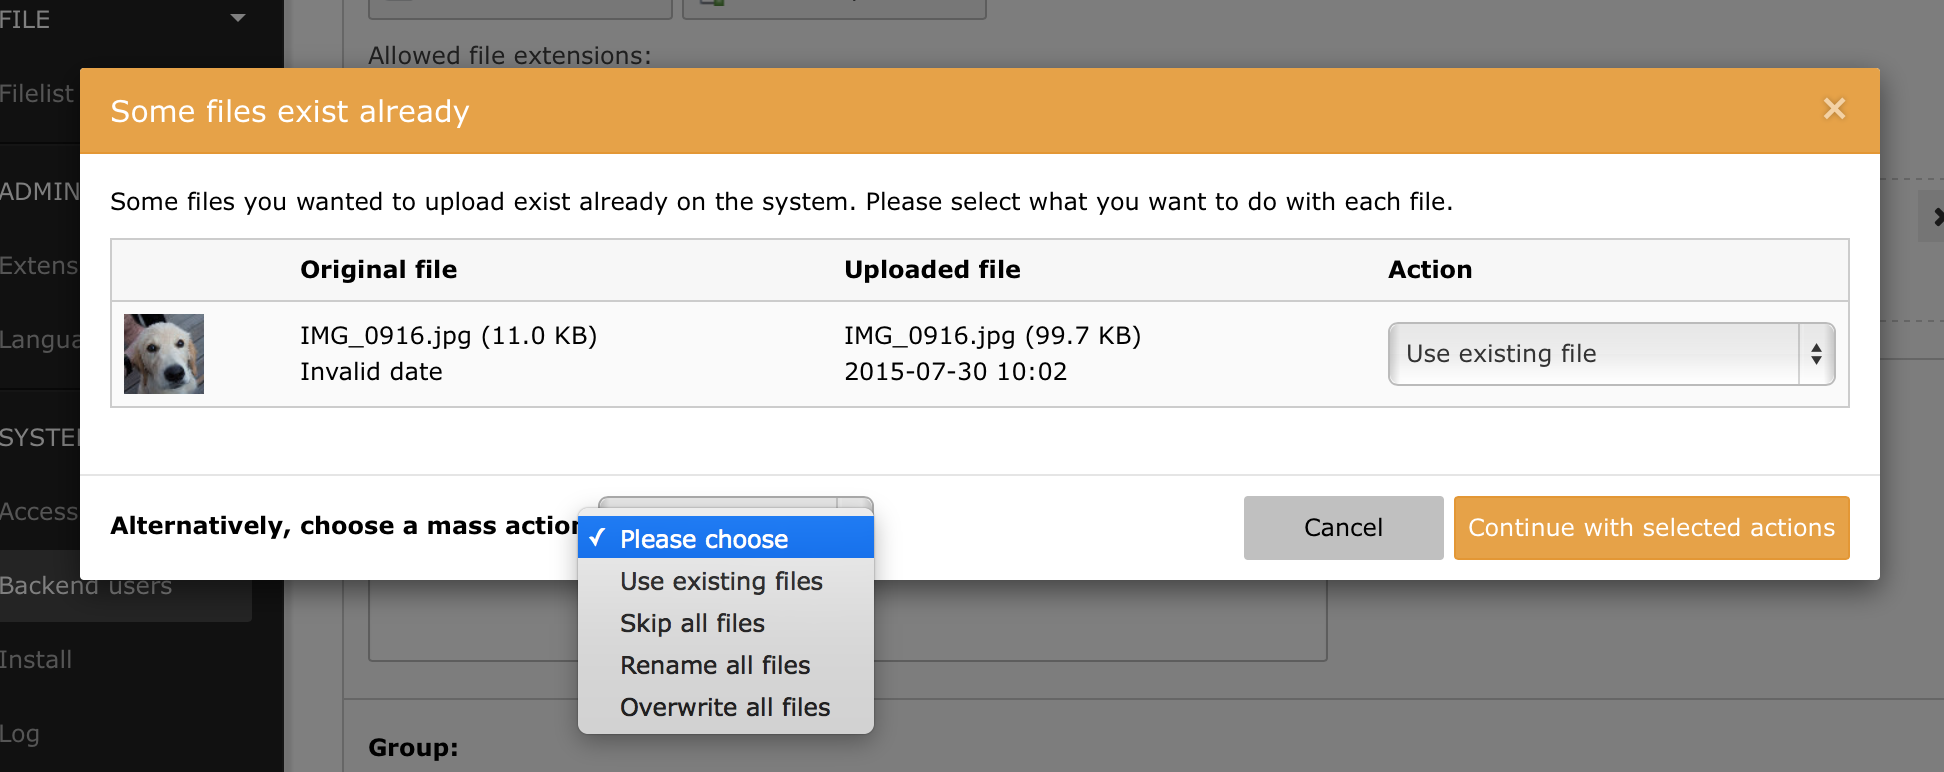
\includegraphics[width=0.9\linewidth]{BackendUserInterface/68197.png}
	\end{figure}

\end{frame}


% ------------------------------------------------------------------------------
% LTXE-SLIDE-START
% LTXE-SLIDE-UID:		dd33b99c-57d16e6f-32c0b034-d4b84ebc
% LTXE-SLIDE-ORIGIN:	31d7dd8e-a3c71be4-309850ab-45a7db72 English
% LTXE-SLIDE-ORIGIN:	f4baa7b8-2237ad1d-5c4be365-a845f207 German
% LTXE-SLIDE-TITLE:		Feature: #68218 - Lock edit for tt_content
% LTXE-SLIDE-REFERENCE:	Feature-68218-LockEditForTt_content.rst
% ------------------------------------------------------------------------------
\begin{frame}[fragile]
	\frametitle{Interfaccia utente Backend}
	\framesubtitle{Modifica limitata agli elementi di contenuto}

	La modifica degli elementi di contenuto può essere limitata agli amministratori
	(simile alla funzione "Blocca la modifica ai non-amministratori" nelle pagine).

	\begin{figure}
		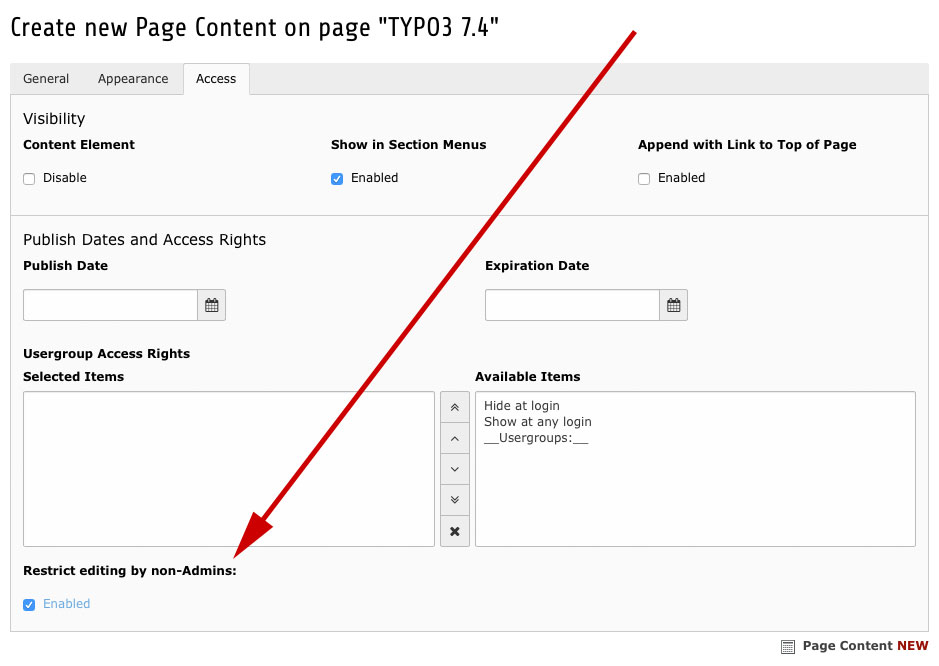
\includegraphics[width=0.6\linewidth]{BackendUserInterface/68218.jpg}
	\end{figure}

\end{frame}

% ------------------------------------------------------------------------------
% LTXE-SLIDE-START
% LTXE-SLIDE-UID:		a67b68b4-25aa500e-f3bb526b-d8fd928c
% LTXE-SLIDE-ORIGIN:	4e60055a-266e3e24-7baa1613-1226575e English
% LTXE-SLIDE-ORIGIN:	bc83e40f-9b7bac03-ea5f07c4-be27eb56 German
% LTXE-SLIDE-TITLE:		Feature: #68315 - Include pageTSconfig file (1)
% LTXE-SLIDE-REFERENCE:	Feature-68315-IncludeAPageTSconfigFileInPagePropertiesLikeTSStaticTemplates.rst
% ------------------------------------------------------------------------------
\begin{frame}[fragile]
	\frametitle{Interfaccia utente Backend}
	\framesubtitle{Inclusione statica di file TSconfig (1)}

	Nelle proprietà della pagina un opzione permette di includere un file TSconfig di pagina
	(stessa cosa dell'inclusioni di template statici TypoScript).

	\begin{figure}
		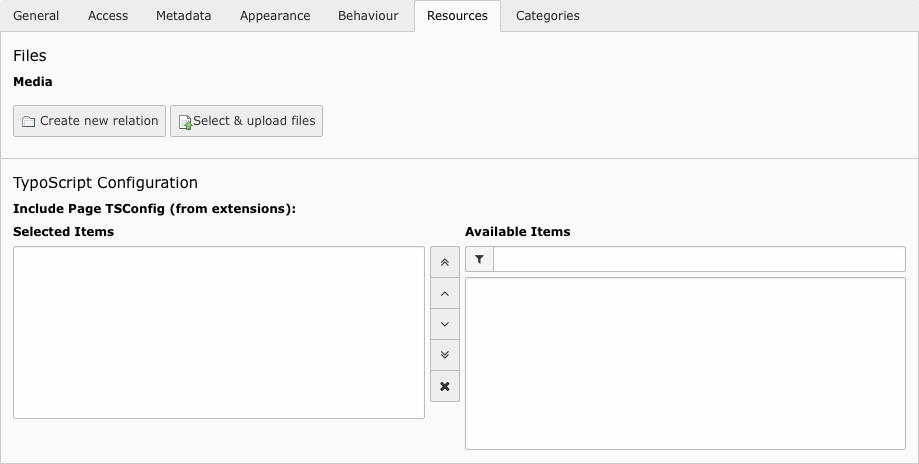
\includegraphics[width=0.8\linewidth]{BackendUserInterface/68315.png}
	\end{figure}

\end{frame}

% ------------------------------------------------------------------------------
% LTXE-SLIDE-START
% LTXE-SLIDE-UID:		f323e939-81c4c633-32be9554-9da22cd5
% LTXE-SLIDE-ORIGIN:	4f5cb411-3ea84dfd-84edb16d-433b9fc5 English
% LTXE-SLIDE-ORIGIN:	9b7bac03-ea5f07c4-be27eb56-ac03e27e German
% LTXE-SLIDE-TITLE:		Feature: #68315 - Include pageTSconfig file (2)
% LTXE-SLIDE-REFERENCE:	Feature-68315-IncludeAPageTSconfigFileInPagePropertiesLikeTSStaticTemplates.rst
% ------------------------------------------------------------------------------
\begin{frame}[fragile]
	\frametitle{Interfaccia utente Backend}
	\framesubtitle{Inclusione statica di file TSconfig (2)}

	% decrease font size for code listing
	\lstset{basicstyle=\tiny\ttfamily}

	Il metodo seguente carica un file TSconfig di pagina:

	\begin{lstlisting}
		\TYPO3\CMS\Core\Utility\ExtensionManagementUtility::registerPageTSConfigFile(
		  'extension_name',
		  'Configuration/PageTS/myPageTSconfigFile.txt',
		  'My special configuration'
		);
	\end{lstlisting}

\end{frame}

% ------------------------------------------------------------------------------
% LTXE-SLIDE-START
% LTXE-SLIDE-UID:		f7158b3d-4ddcfade-fa243ed7-fcac9eeb
% LTXE-SLIDE-ORIGIN:	c00b2bfd-2c1b02b0-a7ef9cd0-62f147d2 English
% LTXE-SLIDE-ORIGIN:	f8d888b1-b93dcf4a-e20b976e-9a5c277e German
% LTXE-SLIDE-TITLE:		Feature: #68395 - Allow real copies of content elements into foreign languages
% LTXE-SLIDE-REFERENCE:	Feature-68395-AllowRealCopiesOfContentElementsIntoForeignLanguages.rst
% ------------------------------------------------------------------------------
\begin{frame}[fragile]
	\frametitle{Interfaccia utente Backend}
	\framesubtitle{Copie reali degli elementi di contenuto}

	E' stato aggiunto un nuovo bottone ad ogni colonna nel modulo "Pagina" che permette una copia \textit{reale} 
	degli elementi di contenuto in una lingua (non solo una referenza).

	\begin{figure}
		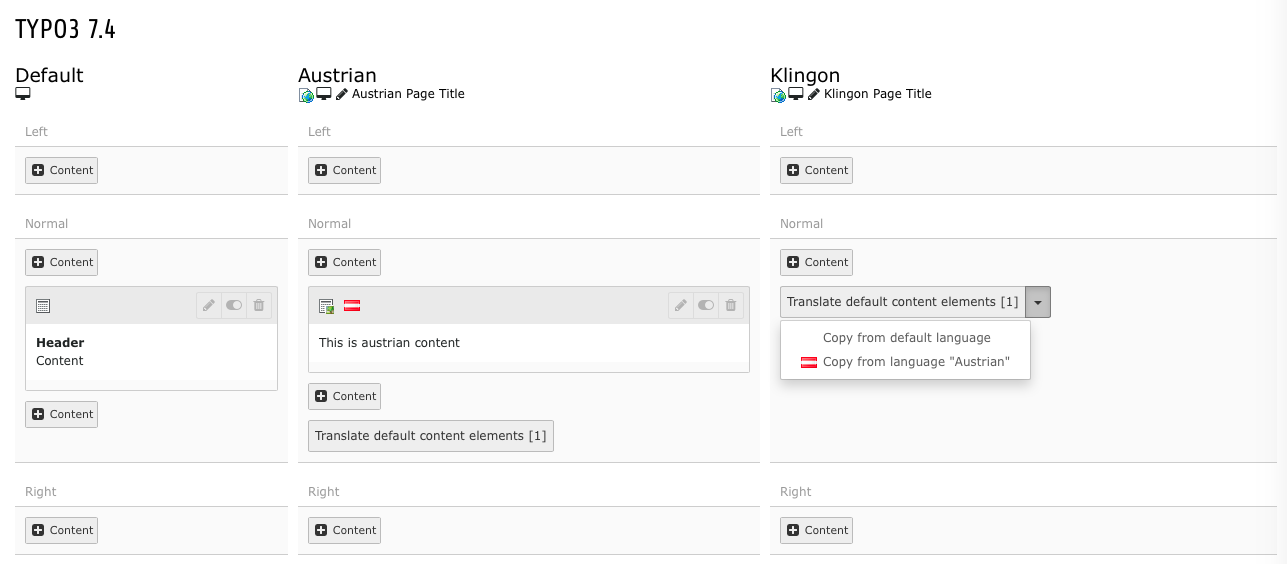
\includegraphics[width=0.9\linewidth]{BackendUserInterface/68395.png}
	\end{figure}

\end{frame}


